	\documentclass[a4paper,twoside,11pt]{article}
\usepackage{a4wide,graphicx,fancyhdr,amsmath,amssymb,float,longtable,chronology,caption,subcaption,appendix}
\usepackage{algorithmic}
\usepackage{hyperref}
\usepackage{listings}
\usepackage{url}
\usepackage{pgffor}
\usepackage{color}

%----------------------- Macros and Definitions --------------------------

\definecolor{mygreen}{rgb}{0,0.6,0}
\definecolor{mygray}{rgb}{0.5,0.5,0.5}
\definecolor{mymauve}{rgb}{0.58,0,0.82}

\lstset{ %
  backgroundcolor=\color{white},   % choose the background color; you must add \usepackage{color} or \usepackage{xcolor}
  basicstyle=\footnotesize,        % the size of the fonts that are used for the code
  breakatwhitespace=false,         % sets if automatic breaks should only happen at whitespace
  breaklines=true,                 % sets automatic line breaking
  captionpos=b,                    % sets the caption-position to bottom
  commentstyle=\color{mygreen},    % comment style
  deletekeywords={...},            % if you want to delete keywords from the given language
  escapeinside={\%*}{*)},          % if you want to add LaTeX within your code
  extendedchars=true,              % lets you use non-ASCII characters; for 8-bits encodings only, does not work with UTF-8
  frame=single,	                   % adds a frame around the code
  keepspaces=true,                 % keeps spaces in text, useful for keeping indentation of code (possibly needs columns=flexible)
  keywordstyle=\color{blue},       % keyword style
 % language=mcrl2,                 % the language of the code
  otherkeywords={*,...},           % if you want to add more keywords to the set
  numbers=left,                    % where to put the line-numbers; possible values are (none, left, right)
  numbersep=5pt,                   % how far the line-numbers are from the code
  numberstyle=\tiny\color{mygray}, % the style that is used for the line-numbers
  rulecolor=\color{black},         % if not set, the frame-color may be changed on line-breaks within not-black text (e.g. comments (green here))
  showspaces=false,                % show spaces everywhere adding particular underscores; it overrides 'showstringspaces'
  showstringspaces=false,          % underline spaces within strings only
  showtabs=false,                  % show tabs within strings adding particular underscores
  stepnumber=2,                    % the step between two line-numbers. If it's 1, each line will be numbered
  stringstyle=\color{mymauve},     % string literal style
  tabsize=2,	                   % sets default tabsize to 2 spaces
 % title=\lstname                   % show the filename of files included with \lstinputlisting; also try caption instead of title
}


\setlength\headheight{20pt}
\addtolength\topmargin{-10pt}
\addtolength\footskip{20pt}

\newcommand{\N}{\mathbb{N}}
\newcommand{\ch}{\mathcal{CH}}
\everymath{\displaystyle}
\newcommand{\define}[2]{\noindent{\bf #1}}
\newcommand{\scg}{System Validation}

\newcommand{\action}[2]{{\tt #1(#2)}}
\newcommand{\todo}[1]{{\color{red}#1}}

\fancypagestyle{plain}{%
	\fancyhf{}
	\fancyhead[LO,RE]{\sffamily\bfseries\large Technische Universiteit Eindhoven}
	\fancyhead[RO,LE]{\sffamily\bfseries\large 2IMF30 \scg}
	\fancyfoot[LO,RE]{\sffamily\bfseries\large Department of Mathematics and Computer Science}
	\fancyfoot[RO,LE]{\sffamily\bfseries\thepage}
	\renewcommand{\headrulewidth}{0pt}
	\renewcommand{\footrulewidth}{0pt}
}

\pagestyle{fancy}
\fancyhf{}
\fancyhead[RO,LE]{\sffamily\bfseries\large Technische Universiteit Eindhoven}
\fancyhead[LO,RE]{\sffamily\bfseries\large 2IMF30 - System Validation}
\fancyfoot[LO,RE]{\sffamily\bfseries\large Department of Mathematics and Computer Science}
\fancyfoot[RO,LE]{\sffamily\bfseries\thepage}
\renewcommand{\headrulewidth}{1pt}
\renewcommand{\footrulewidth}{0pt}

%-------------------------------- Title ----------------------------------

\title{\sffamily\bfseries 2IMF30 \scg\ - Project 1}
\author{Tom van Diggelen \qquad Student number: 0745801 \\{\tt t.w.t.v.diggelen@student.tue.nl}\\ \\ Huib Donkers \qquad Student number: 0769015 \\{\tt h.t.donkers@student.tue.nl} \\ \\ Jeroen Noten \qquad Student number: 0784113 \\{\tt j.f.h.noten@student.tue.nl}\\ \\ Mart Pluijmaekers \qquad Student number: 0753117 \\{\tt m.h.l.pluijmaekers@student.tue.nl} \\ \\ Hein van Beers \qquad Student number: 0765658 \\{\tt h.a.v.beers@student.tue.nl}}

\date{\today}

\allowdisplaybreaks

%--------------------------------- Text ----------------------------------

\begin{document}
\maketitle
\tableofcontents

\newpage
\section{Introduction}
% !TEX root = ../report.tex
This document contains the design of a controller for an embeded controller for a wafer stepper. The purpose was to design the controller such that it can be proven to comply with all set requirements which had been formulated in advance.\\

At first, we will give a short textual description of the system that we chose to design and implement. After that we will give a list of requirements for the whole system, that we derived from the stated description. These requirements are described in natural language. When we have settled all the requirements, we continue with identifying the interactions that are relevant to the system. We describe clearly but compactly the meaning of each interaction in words, together with its desired parameters. When the interactions have been described, we can start with translating all the global requirements in terms of these interactions. When the requirements have been described in this manner, we can start using the modal $\mu$-calculus to convert the requirements into modal formulas with which we can verify the system. After this, we will describe the behaviour of all controllers in the architecture using mCRL2 \cite{url:mcrl}. This gives a short overview of all the parallel processes that communicate in our system. Finally, we will argue which requirements we have verified and which requirements we were unable to verify.

\section{Assignment description}
We designed a controller for an EUV (Extreme Ultra Violet) ASML waferstepper. This controller takes care of the logistics of silicon wafers in the waferstepper. If a rack of wafers arrives at an EUV waferstepper, they must enter the machine one by one through a sluice. There are two sluices, such that if one of the two sluices does not function the other can be used to let wafers enter and leave the machine.

There is one robot which picks wafers from the input rack and puts them into one of the two sluices. There is another robot inside the machine which takes wafers from the sluices and puts them into a waiting rack. A third robot moves the wafers from the waiting rack to the image projection system and moves them back to another waiting rack after an image has been projected. The wafers are subsequently moved through a sluice to the outside of the machine and to an output rack. The layout of the waferstepper is shown in figure~\ref{fig:stepperlayout}.

\begin{figure}[h]
    \centering
	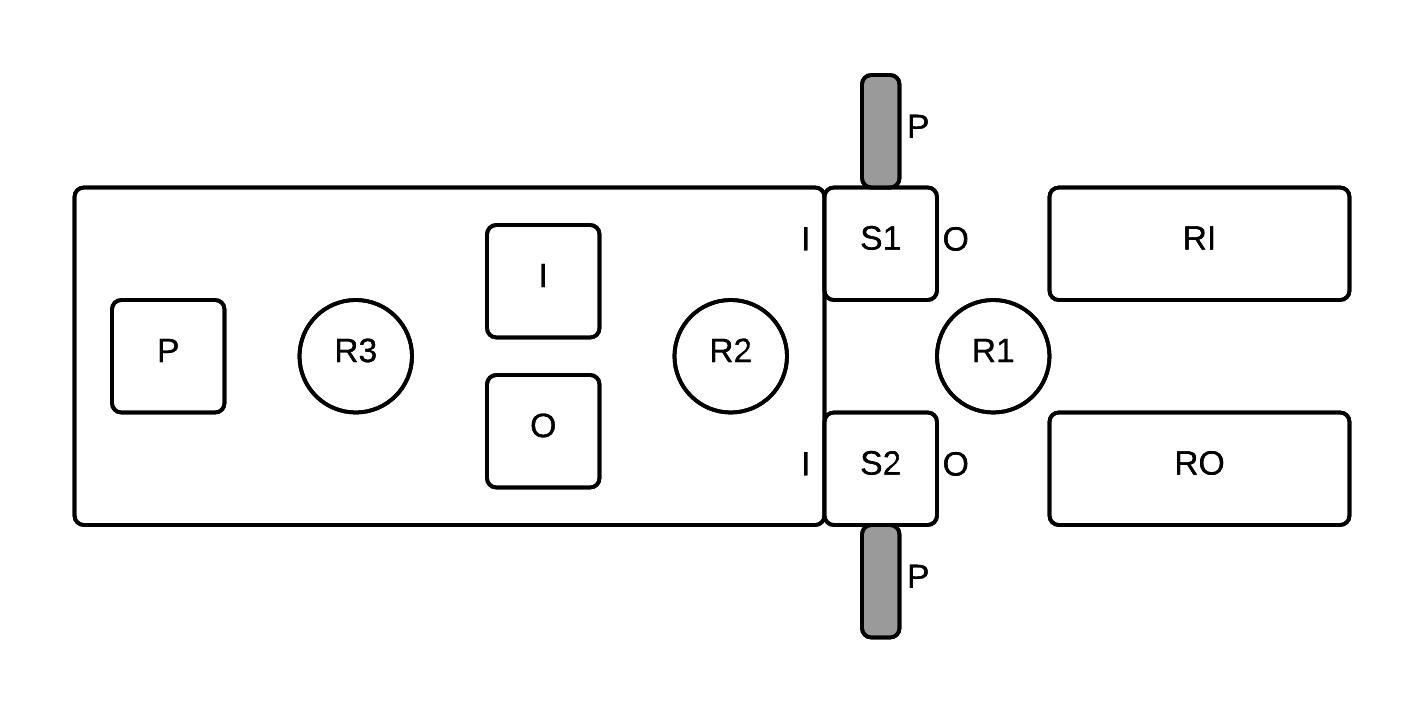
\includegraphics[width=0.6\textwidth]{waferstepper.png}
	\caption{The layout of the waferstepper.\\
	P: Projector\\R3: Robot that places wafers under the projector\\
	I: Waiting rack for unprocessed wafers\\
	O: Waiting rack for processed wafers\\
	R2: Robot that moves wafers from sluices to the waiting racks and vice versa\\
	S1 and S2: Sluices, each sluice has an inside door I, an outside door O and a pump P\\
	R1: Robot that moves wafers from the input rack to the sluices and from the sluices to the output rack\\
	RI: Wafer input rack\\
	RO: Wafer output rack}
	\label{fig:stepperlayout}
\end{figure}

The controller we design may not in any case perform harmful actions causing damage to the expensive waferstepper. The controller may not, for example, place wafers into a sluice when its doors are closed. Similarly it may not pick a wafer from a sluice with closed doors or from the projector while the wafer is begin projected. Additionally the controller should not place wafers on top of each other.

The doors of the sluices are less reliable and can get stuck. This is not something the controller can prevent, so it has to deal with broken doors and continue to operate even when a sluice is out of order. When this happens, the other sluice must be used to move wafers both into as out of the machine.

\section{Basic requirements}
% !TEX root = ../report.tex
\subsection{Definitions}
\begin{enumerate}
  \item A wafer is considered processed when the projector has finished processing and the wafer has exited the stepper.
\end{enumerate}

\subsection{Assumptions}
\begin{enumerate}
  \item The doors are the only part of the machines that can malfunction.
  \item The main room is assumed to always be a vacuum.
  \item The external input and output racks are assumed to be infinite in size.
  \item Sluice pumps change the air pressure to either zero or one atmosphere.
\end{enumerate}

\subsection{Requirements}
\begin{enumerate}
  \item At least one door of a sluice is closed at any point in time.
  \item No robot may interact with a sluice whenever its access door is closed.
  \item An unprocessed wafer will eventually be processed.
  \item Internal racks, sluices, and the projector place each contain at most one wafer.
  \item When the projector is at work, no interaction with the wafer is permissible.
  \item A sluice door cannot open until the pressure on both sides is equal.
  \item Sluice pumps will not operate until both of its doors are closed.
  \item \todo{Restricties voor robots toevoegen}
\end{enumerate}


\section{Actions}
\begin{tabular}{|l|l|l|p{4cm}|}
\hline  
  \textbf{Action} & \todo{\textbf{Executed by}} & \textbf{Variables} & \textbf{Meaning} \\
  \hline
  \todo{\action{get}{$p$}} & Robots & $p$: A place in the system & Get a wafer from place $p$\\
  \hline
  \todo{\action{put}{$p$}} & Robots & $p$: A place in the system & Put a wafer on place $p$\\
  \hline
  \action{project}{} & Projector & None & Project a wafer\\
  \hline
  \action{openInside}{$s$} & Inside sluice doors & $s$: The corresponding sluice & Open the inside sluice door of sluice $s$\\
  \hline
  \action{openOutside}{$s$} & Outside sluice doors & $s$: The corresponding sluice & Open the outside sluice door of sluice $s$\\
  \hline
  \action{closeInside}{$s$} & Inside sluice doors & $s$: The corresponding sluice & Close the inside sluice door of sluice $s$\\
  \hline
  \action{closeOutside}{$s$} & Outside sluice doors & $s$: The corresponding sluice & Close the outside sluice door of sluice $s$\\
  \hline
  \action{Vacuum}{$s$} & Pumps & $s$: The corresponding sluice & Make sluice $s$ into a vacuum\\
  \hline
  \action{deVacuum}{$s$} & Pumps & $s$: The corresponding sluice & Make sluice $s$ into normal air pressure\\
  \hline
  \action{read}{$s$} & Sensors & $s$: The corresponding sluice & Read the value of the sensor in sluice $s$\\
  \hline
\end{tabular}

\section{Requirements in terms of actions}
% !TEX root = ../report.tex

\begin{description}
 \item[1. At least one door of a sluice is closed at any point in time] \hfill \\
 For any sluice $s$:
 \begin{itemize}
  \item Between any \action{openInside}{$s$} and its most recent preceding \action{openOutside}{$s$}, there must be a \action{closeOutside}{$s$}
  \item Between any \action{openOutside}{$s$} and its most recent preceding \action{openInside}{$s$}, there may not be a \action{closeInside}{$s$}
 \end{itemize}

 \item[2. No robot may interact with a sluice whenever its access door is closed] \hfill \\
For any sluice $s$:

\begin{itemize}
	\item Between any \action{move}{$RI, s$} and its most recent preceding \action{closeOutside}{$s$}, there must be a \action{openOutside}{$s$}.
	\item between any \action{move}{$s, a$} with $a \in \{ I, O \}$ and its most recent preceding \action{closeInside}{$s$}, there must be a \action{openInside}{$s$}.
	\item between any \action{move}{$a, s$} with $a \in \{ I, O \}$ and its most recent preceding \action{closeInside}{$s$}, there must be a \action{openInside}{$s$}.
	\item between any \action{move}{$s, a$} with $a \in \{ RI, RO \}$ and its most recent preceding \action{closeOutside}{$s$}, there must be a \action{openOutside}{$s$}.
\end{itemize}
 
 \item[\smash{\shortstack[l]{3. Any wafer in the system will eventually be processed unless the system breaks,\\ or the wafer is inside a sluice when the sluice itself breaks}}] \hfill 
 \begin{itemize}
 \item There must be at least one \action{detectInputWafer}{$s$} for some status $s$.
 \item After any \action{detectInputWafer}{$s$} for some status $s$ there must be at least one \action{detectInputWafer}{$t$} for some status $t$.
 \item After any \action{detectInputWafer}{$s$} there must be a \action{move}{$RI, a$} for some place $a$ in the system.
 \item After any \action{move}{$RI, a$} for some place $a$ in the system, there must be a \action{move}{$b, RO$} for some place $b$ in the system.
 \end{itemize}
 
 
\item[4. Internal racks, sluices and the projector each contain at most one wafer] \hfill \\
For any internal place $p_i \in \{S1, S2, I, O, P\}$ and any three places $p_1, p_2, p_3 \in \{S1, S2, I, O, P, RI, RO\}$: between any \action{move}{$p_1, p_i$} and its most recent preceding \action{move}{$p_2, p_i$}, there must be a \action{move}{$p_i, p_3$}. 
 
\item[5. When the projector is at work, no interaction with the wafer is permissible] \hfill \\
For any place $p$: between any \action{move}{$P, p$} or \action{move}{$p, P$} and its most recent preceding \action{beginProject}{}, there must be a \action{endProject}{}. 
 
 \item[6. A sluice door cannot open until the pressure on both sides is equal] \hfill \\
 For any sluice $s$:
 \begin{itemize}
  \item Between any \action{openInside}{$s$} and its most recent preceding \action{deVacuum}{$s$}, there must be a \action{Vacuum}{$s$}
  \item Between any \action{openOutside}{$s$} and its most recent preceding \action{Vacuum}{$s$}, there must be a \action{deVacuum}{$s$}
 \end{itemize}

 \item[7. Sluice pumps cannot operate until both of its doors are closed] \hfill \\
 For any sluice $s$:
 \begin{itemize}
  \item Between any \action{Vacuum}{$s$} or \action{deVacuum}{$s$} and its most recent preceding \action{openInside}{$s$}, there must be a \action{closeInside}{$s$}
  \item Between any \action{Vacuum}{$s$} or \action{deVacuum}{$s$} and its most recent preceding \action{openOutside}{$s$}, there must be a \action{closeOutside}{$s$}
 \end{itemize}

\item[8. No robot can place a projected wafer in $RI$] \hfill \\
For any place $a$ in the system: a \action{move}{$a, RI$} may only be executed when $position(a) = \texttt{unprojected}$.

\item[9. No robot can place an unprojected wafer in $RO$] \hfill \\
For any place $a$ in the system: a \action{move}{$a, RO$} may only be executed when $position(a) = \texttt{projected}$.

\item[10. No robot can take a wafer from $RO$] \hfill \\
\action{move}{$RO, a$} cannot take place for any $a$.
 
\end{description}


\section{Requirements in modal $\mu$-calculus}
% !TEX root = ../report.tex

\newcommand{\tab}{\hspace{1em}}

\begin{description}
 \item[1. At least one door of a sluice is closed at any point in time]\mbox{}\\
\[
[true^*]\forall s:Sluice,d:Door.[openDoor(d, s).\overline{closeDoor(d, s)}^*.openDoor(d, s)]false
\]


 \item[2. No robot may interact with a sluice whenever its access door is closed]\mbox{}\\
\begin{align*}
& [true^*]\forall s:Sluice.( \\
& \tab [closeDoor(outsideDoor, s).(\overline{openDoor(outsideDoor, s)}^*.( \\
& \tab\tab move(RI, sluicePlace(s)) \cup move(sluicePlace(s), RI) \cup \\
& \tab\tab move(RO, sluicePlace(s)) \cup move(sluicePlace(s), RO) \\
& \tab )]false \wedge \\
& \tab [closeDoor(insideDoor, s).(\overline{openDoor(insideDoor, s)}^*.( \\
& \tab\tab move(I, sluicePlace(s)) \cup move(sluicePlace(s), I) \cup \\
& \tab\tab move(O, sluicePlace(s)) \cup move(sluicePlace(s), O) \\
& \tab )]false \\
& )
\end{align*}
 
 \item[3. Any wafer in the system will eventually be processed]

	\begin{align*}
& [true^*.detectInputWafer] \mu X( \\
&          \tab                          position: Place = RI,    \\  
&          \tab                          projecting: Bool = false,  \\
&          \tab                          projected: Bool = false,   \\
&          \tab                          stuck: Bool = false,       \\
&          \tab                          brokenDoors: SluiceDoor \to Bool = nothingBroken   \\
&                                 ).( \\
&  \tab ( \\
&  \tab\tab  \forall a,b:Place.[move(a,b)]X( \\
&  \tab\tab  \tab                              if(a \approx position, b, position), \\
&  \tab\tab  \tab                              projecting \wedge a \not \approx position, \\
&  \tab\tab  \tab                              projected, \\
&  \tab\tab  \tab                              if(a \approx position \wedge \exists s:Sluice . sluicePlace(s) \approx b \wedge ( \\
& \tab\tab\tab\tab (\neg projected \wedge brokenDoors(sluiceDoor(s, insideDoor))) \\ 
& \tab\tab\tab\tab \vee (projected \wedge brokenDoors(sluiceDoor(s, outsideDoor))) \\
& \tab\tab\tab ), true, stuck), \\
&  \tab\tab  \tab                              brokenDoors \\
&  \tab\tab                               ) \\
&  \tab\tab  \wedge [\overline{(\exists a,b:Place.move(a,b)) \cup beginProject \cup endProject} \\
& \tab\tab\tab\tab \overline{ \cup (\exists d:Door,s:Sluice.doorStuck(d, s))}]X( \\
& \tab\tab\tab\tab\tab\tab position, projecting, projected, stuck, brokenDoors) \\
&  \tab\tab  \wedge [beginProject]X(position, position \approx P, projected, stuck, brokenDoors)
&  \tab\tab  \wedge [endProject]X(position, false, projected \vee (projecting \wedge position \approx P), stuck, brokenDoors) \\
&  \tab\tab  \wedge \forall d:Door,s:Sluice.[doorStuck(d, s)]X( \\
&  \tab\tab                        \tab                        position, \\
&  \tab\tab                        \tab                        projecting, \\
&  \tab\tab                        \tab                        projected, \\
&  \tab\tab                        \tab                        if(sluicePlace(s) \approx position \wedge ((\neg projected \wedge d == insideDoor) \\
& \tab\tab\tab\tab\tab \vee (projected \wedge d == outsideDoor)), true, stuck), \\
&  \tab\tab                       \tab brokenDoors[sluiceDoor(s,d)\to true] \\
&  \tab\tab                                              ) \\
&  \tab ) \\
&  \vee (position \approx RO \wedge projected) \vee stuck \\
&)
	\end{align*}

 
 \item[4. Internal racks, sluices and the projector each contain at most one wafer]
    
\begin{align*}
		&[true*] \nu X(status:Place \to WaferState=emptyPlaces).(\\
  & \tab\tab [\overline{((\exists a,b:Place.move(a,b)) \cup detectInputWafer)}]X(status)\\
  & \tab\tab  \wedge [detectInputWafer]X(status[RI \to unprojected])\\
  & \tab\tab  \wedge \forall a,b:Place.[move(a, b)](val(status(a) != empty \implies status(b)  == empty) \wedge \\ & \tab \tab X(status[b \to status(a)][a \to empty]))\\
&)
	\end{align*}

 
 \item[5. When the projector is at work, no interaction with the wafer is permissible]
 	\begin{align*}
 		&[true^*.beginProject().\overline{endProject()}^*.move(P,O)]false
	\end{align*}
	
 \item[6. A sluice door cannot open until the pressure on both sides is equal]
%		&[true^*.vacuum(s).stopPumping(s).\overline{readAirPressure(s,0)^*}.openInside(s)]false \\
%		&[true^*.deVacuum(s).stopPumping(s).\overline{readAirPressure(s,1)^*}.openOutside(s)]false \\
	\begin{align*}
&[true^*]\forall s:Sluice . ( \\
&\tab  [vacuum(s).stopPumping(s).\overline{readAirPressure(s, vacuum)}^*\\
&\tab\tab\tab.openDoor(insideDoor,s)]false \\
&\tab  \wedge [deVacuum(s).stopPumping(s).\overline{readAirPressure(s, normal)}^*\\
&\tab\tab\tab.openDoor(outsideDoor,s)]false \\
&)		
	\end{align*}
	
 \item[7. Sluice pumps cannot operate until both of its doors are closed]
 
  For $s \in \{sluice1, sluice2\}:$
 \begin{align*}
		&[true^*.openInside(s).\overline{closeInside(s)^*}.vacuum(s)]false \\
		&[true^*.openInside(s).\overline{closeInside(s)^*}.deVacuum(s)]false \\
		&[true^*.openOutside(s).\overline{closeOutside(s)^*}.vacuum(s)]false \\
		&[true^*.openOutside(s).\overline{closeOutside(s)^*}.deVacuum(s)]false \\
	\end{align*}

 \item[8. No robot can place a projected wafer in $RI$]\mbox{}\\
$
[true^* \cdot detectInputWafer]\\
\nu X(position:Place=RI, projecting:Bool=false, projected:Bool=false)\\
.\forall a,b:Place.[move(a,b)]X(if(a \approx position, b, position), projecting \wedge a \not \approx position, projected)\\
\wedge [\overline{\exists a,b:Place.move(a,b) \cup beginProject \cup endProject)}]X(position, projecting, projected)\\
\wedge [beginProject]X(position, position \approx P, projected)\\
\wedge [endProject]X(position, false, projected \vee (projecting \wedge position \approx P))\\
\wedge (position \approx RI \implies \neg projected)
$
 \item[9. No robot can place an unprojected wafer in $RO$] \mbox{}\\
$
[true^* \cdot detectInputWafer]\\
\nu X(position:Place=RI, projecting:Bool=false, projected:Bool=false)\\
.\forall a,b:Place.[move(a,b)]X(if(a \approx position, b, position), projecting \wedge a \not \approx position, projected)\\
\wedge [\overline{\exists a,b:Place.move(a,b) \cup beginProject \cup endProject)}]X(position, projecting, projected)\\
\wedge [beginProject]X(position, position \approx P, projected)\\
\wedge [endProject]X(position, false, projected \vee (projecting \wedge position \approx P))\\
\wedge (position \approx RO \implies projected)
$

 \item[10. No robot can take a wafer from $RO$]

\[
	\forall p:Place . [true^* \cdot move(RO, p)]false
\]

\end{description}


\section{Automaton defined in mCRL2}
% !TEX root = ../report.tex

Our model consists of 7 parallel processes that communicate.
\begin{enumerate}
 \item Two identical processes managing a single sluice each. They control the sluice doors and the pumps and communicate with the robots about whether or not they may reach into the sluice.
 \item A process controlling $R3$ and the projector.
 \item A process controlling $R2$.
 \item A process controlling $R1$.
 \item Position tracker, which tracks the positions and state of each wafer. This process communicates with the three processes controlling the robots and projector, both in order to track the wafer, as well as to prevent the robots from making illegal moves (e.g. placing a token on an occupied rack).
 \item A safeguard process, which monitors the doors. This process itself consists of 4 parallel processes, each monitoring a single door. Each of these processes communicate with the process controlling their door. A safeguard terminates when a door gets stuck, which will prevent the door controlling from moving the stuck door (because it can no longer communicate with the terminated process).
\end{enumerate}


\section{Results}
We have checked the requirements on the model with the mCRL2 tool set. Because checking of some requirements takes very long, we have not obtained all results yet. The results are:
\begin{tabular}{|l|l|}
\hline
Requirement 1 & true \\
\hline
Requirement 2 & true \\
\hline
Requirement 3 & not yet known \\
\hline
Requirement 4 & not yet known \\
\hline
Requirement 5 & true \\
\hline
Requirement 6 & not yet known \\
\hline
Requirement 7 & true \\
\hline
Requirement 8 & not yet known \\
\hline
Requirement 9 & not yet known \\
\hline
Requirement 10 & true \\
\hline
\end{tabular}

\section{Conclusion}
% !TEX root = ../report.tex

Conclusion here

\begin{thebibliography}{9}
\bibitem{url:mcrl}
http://www.mcrl2.org/

\end{thebibliography}

\newpage
\begin{appendices}
\section{mCRL2 model}
\lstinputlisting{../model/model.mcrl2}

\newpage
\section{mCRL2 requirements}

\foreach \n in {1,...,10}{
	\subsection{Requirement: \n}
	\lstinputlisting{../model/Requirements/Requirement\n.mcf}
}


\end{appendices}


\end{document}
